\documentclass[cs4size,a4paper]{ctexart}   
%==================== 数学符号公式 ============
\usepackage{amsmath}                 % AMS LaTeX宏包
\usepackage[style=1]{mdframed}
\usepackage{amsthm}
\usepackage{amsfonts}
\usepackage{mathrsfs}                % 英文花体字 体
\usepackage{bm}                      % 数学公式中的黑斜体
\usepackage{bbding,manfnt}           % 一些图标,如 \dbend
\usepackage{lettrine}                % 首字下沉,命令\lettrine
\def\attention{\lettrine[lines=2,lraise=0,nindent=0em]{\large\textdbend\hspace{1mm}}{}}
\usepackage{longtable}
\usepackage[toc,page]{appendix}
\usepackage{geometry}                % 页边距调整
\geometry{top=3.0cm,bottom=2.7cm,left=2.5cm,right=2.5cm}
%====================公式按章编号==========================
\numberwithin{equation}{section}
\numberwithin{table}{section}
\numberwithin{figure}{section}
%================= 基本格式预置 ===========================
\usepackage{fancyhdr}
\pagestyle{fancy}
\fancyhf{}  
\fancyhead[C]{\zihao{5}  \kaishu 北邮SDN大赛报告模板}
\fancyfoot[C]{~\zihao{5} \thepage~}
\renewcommand{\headrulewidth}{0.65pt} 
\CTEXsetup[format={\centering\bfseries\zihao{-2}},name={第, 章}]{section}
\CTEXsetup[nameformat={\bfseries\zihao{3}}]{subsection}
\CTEXsetup[nameformat={\bfseries\zihao{4}}]{subsubsection}
%================== 图形支持宏包 =========================
\usepackage{subfigure}
\usepackage{graphicx}                % 嵌入png图像
\usepackage{color,xcolor}            % 支持彩色文本、底色、文本框等
\usepackage{hyperref}                % 交叉引用
\usepackage{caption}
\captionsetup{figurewithin=section}
%==================== 源码和流程图 =====================
\usepackage{listings}                % 粘贴源代码
\usepackage{xcolor}
\usepackage{color}
\definecolor{dkgreen}{rgb}{0,0.6,0}
\definecolor{gray}{rgb}{0.5,0.5,0.5}
\definecolor{mauve}{rgb}{0.58,0,0.82}
 \usepackage{xcolor}
 \lstset{
  %行号
    numbers=left,
    %背景框
    framexleftmargin=8mm,
    frame=none,
     %背景色
    %backgroundcolor=\color[rgb]{1,1,0.76},
     backgroundcolor=\color[RGB]{245,245,244},
     %样式
   keywordstyle=\bf\color{blue},
   identifierstyle=\bf,
    numberstyle=\color[RGB]{0,192,192},
    commentstyle=\it\color[RGB]{0,96,96},
   stringstyle=\rmfamily\slshape\color[RGB]{128,0,0},
   %显示空格
    showstringspaces=false
 }


%--------------------
\hypersetup{hidelinks}
\usepackage{booktabs}  
\usepackage{shorttoc}
\usepackage{tabu,tikz}
\usepackage{float}

\usepackage{multirow}



\tabcolsep=1ex
\tabulinesep=\tabcolsep
\newlength\tikzboxwidth
\newlength\tikzboxheight
\newcommand\tikzbox[1]{%
        \settowidth\tikzboxwidth{#1}%
        \settoheight\tikzboxheight{#1}%
        \begin{tikzpicture}
        \path[use as bounding box]
                (-0.5\tikzboxwidth,-0.5\tikzboxheight)rectangle
                (0.5\tikzboxwidth,0.5\tikzboxheight);
        \node[inner sep=\tabcolsep+0.5\arrayrulewidth,line width=0.5mm,draw=black]
                at(0,0){#1};
        \end{tikzpicture}%
        }

\makeatletter
\def\hlinew#1{%
  \noalign{\ifnum0=`}\fi\hrule \@height #1 \futurelet
   \reserved@a\@xhline}
   
\newcommand{\tabincell}[2]{\begin{tabular}{@{}#1@{}}#2\end{tabular}}%

\usepackage{subfigure}

\usepackage{CJK}
\usepackage{ifthen}


\usepackage{graphicx} 
\newcommand{\HRule}{\rule{\linewidth}{0.5mm}}

\newtheorem{Theorem}{定理}
\newtheorem{Lemma}{引理} 
%%使得公式随章节自动编号
\makeatletter
\@addtoreset{equation}{section}
\makeatother
\renewcommand{\theequation}{\arabic{section}.\arabic{equation}}

%-------------------------
	
\usepackage{pythonhighlight}
\usepackage{tikz}                    
\usepackage{tikz-3dplot}
\usetikzlibrary{shapes,arrows,positioning}
%===================   正文开始    ===================
\begin{document}
\bibliographystyle{gbt7714-2005}     %论文引用格式
%===================  定理类环境定义 ===================
\newtheorem{example}{例}              % 整体编号
\newtheorem{algorithm}{算法}
\newtheorem{theorem}{定理}            % 按 section 编号
\newtheorem{definition}{定义}
\newtheorem{axiom}{公理}
\newtheorem{property}{性质}
\newtheorem{proposition}{命题}
\newtheorem{lemma}{引理}
\newtheorem{corollary}{推论}
\newtheorem{remark}{注解}
\newtheorem{condition}{条件}
\newtheorem{conclusion}{结论}
\newtheorem{assumption}{假设}
%==================重定义 ===================
\renewcommand{\contentsname}{目录}     
\renewcommand{\abstractname}{摘要} 
\renewcommand{\refname}{参考文献}     
\renewcommand{\indexname}{索引}
\renewcommand{\figurename}{图}
\renewcommand{\tablename}{表}
\renewcommand{\appendixname}{附录}
\renewcommand{\proofname}{证明}
\renewcommand{\algorithm}{算法} 
%============== 封皮和前言 =================
\newcommand{\chinesethesistitle}{��������ҵ��ѧѧλ����~\LaTeX~ģ��~(\version~��)}
\newcommand{\englishthesistitle}{\LaTeX~Dissertation Template of \\Harbin Institute of Technology~(Version \version)}
\newcommand{\chinesethesistime}{2005~��~6~��}
\newcommand{\englishthesistime}{June, 2005}

\ctitle{��������ҵ��ѧѧλ����\\ \LaTeX~ģ��~(\version~��)}
\cdegree{\cxueke\cxuewei}
\caffil{�������ѧ�뼼��ѧԺ} %����У��������ϵ���ƣ�ͬ��ѧ����Ա�����λ��
\csubject{�����ϵͳ�ṹ}                 %(~������ѧ����д~)
\cauthor{ij~~ij~~ij}
\csupervisor{ij~~ij~~ij~~~~��~~��} %��ʦ����
%\cassosupervisor{ij~~ij~~ij~~~~��~~��}     %(~��������������ʦ���Բ��д���~)
%\ccosupervisor{~ij~~ij~~ij~~~~��~~��~} %(~���޸���ʦ���д���~)
\cdate{\chinesethesistime}

\etitle{\englishthesistitle}
\edegree{\exuewei \ of \exueke}
\esubject{Computer Architecture}
\eauthor{Alice}
\esupervisor{Professor Bob}
%\ecosupervisor{Professor X}
%\eassosupervisor{Professor Y}
\edate{\englishthesistime}

\natclassifiedindex{TP309}  %����ͼ������
\internatclassifiedindex{681.324}  %����ͼ������
\cabstract{
���Ǹ��ݹ�������ҵ��ѧѧλ���Ĺ淶������\LaTeX{}��ʿ����ģ�塣

��ģ��������UFO��(2004)�����廪��ѧ��ʿ����ģ�尴�չ�������ҵ��ѧ��
�Ĺ淶������\LaTeX{}����ģ�壬����cucme��Stanley��TeX��(2005)���ѵ����ƺ���
�ģ�Ŀǰ�Ѿ�``����ȫ��''���������Ĺ淶��Ҫ�󣬵����ɱ���Ļ�����һЩ���⣬
ϣ����Ҽ���Ŭ���Ľ��ͳ�����

��Ȼ���ģ���ļ�������һ����ʼ��
ϣ����``ţ��''�ܹ��ۺ���Щ�����γ�������ģ���ļ���
�츣�Ժ���ֵܽ����ǡ�

��ģ���Ŀ��ּ���ƹ�\LaTeX{}��һ������Ű������ڹ������Ӧ�ã�Ϊ���ͬ
ѧ�ṩһ�����㡢���۵�����ģ�壬��������׫д������鷳��

}

\ckeywords{\LaTeX; ����ģ��}

\eabstract{
This is a \LaTeX{} dissertation template of Harbin Institute of Technology, which is built according to the required format.
}

\ekeywords{\LaTeX; dissertation template}
\makecover
\clearpage

\pagestyle{plain}
\pagenumbering{Roman}
%\section*{\zihao{2} \centering 摘要}
%
%\vskip0.5cm
%本文基于武汉理工大学本科生毕业论文格式2013版的相关要求,结合\LaTeX 在实际运用中的基本技巧和方法对于科技论文排版方法进行一个简略的介绍。通过参照本科生毕业论文的相关要求,实现了符合国际科技论文排版规则的具有一定美感的毕业论文模板设计。 
%
%
%\textbf{关键词:}  动力定位, 船舶操纵性 ,控制方法,状态估计算法
%\addcontentsline{toc}{section}{摘要}
%
%\clearpage
%\section*{\zihao{2} \centering \textbf{Abstract} }
%   %用了Times New Roman字体来美化观感
%
%In this short article we will discuss about \LaTeX\,  for your dissertation \\
%
%\textbf{Key Words:} Dynamic Positioning, Ship Manoeuvrability ,Control Algorithm, State Estimate Algorithm
%\addcontentsline{toc}{section}{Abstract}
%




\pagestyle{empty}
\tableofcontents 
\thispagestyle{empty}
%============== 论文正文   =================
\pagestyle{fancy}
\pagenumbering{arabic}
\section{登录与注册}

\subsection{Home Page}
访问前端首页地址http://localhost:8080/.可以看到如下欢迎页.

\begin{figure}[thbp!]
	\centering
	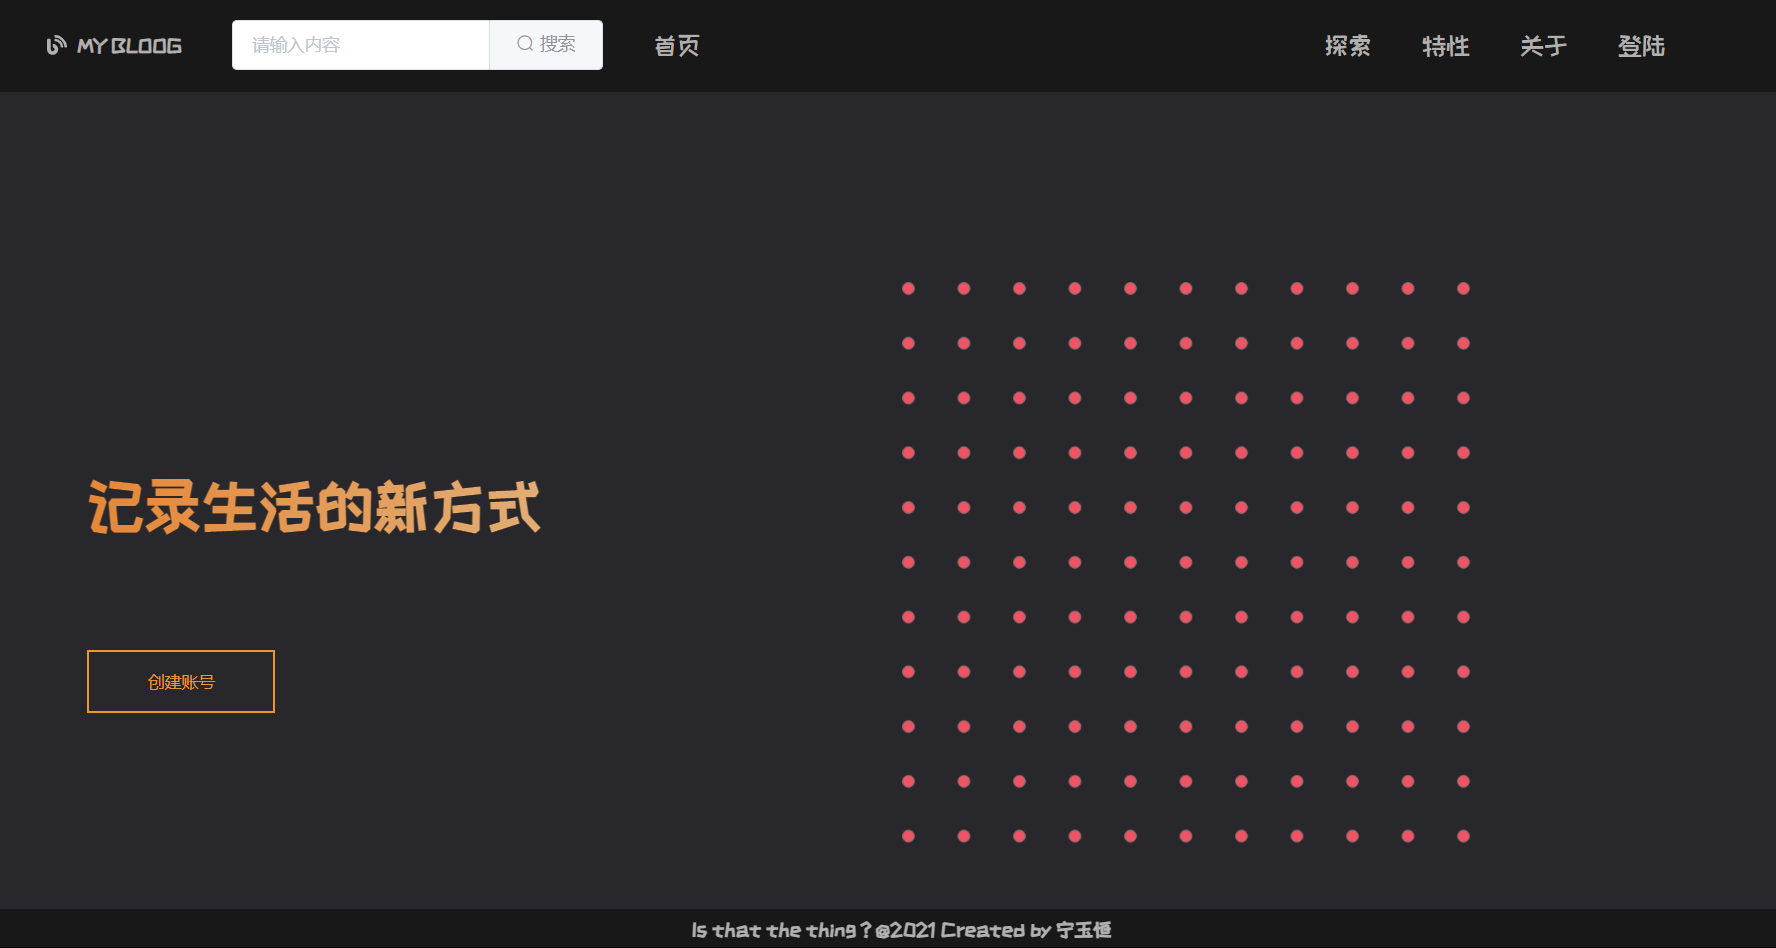
\includegraphics[scale=0.35]{figure/home_page}
	\caption{主页}
\end{figure}

\subsection{注册}
点击首页左侧的创建账号,可以访问注册页,需要上传头像及填写基本信息.

\begin{figure}[thbp!]
	\centering
	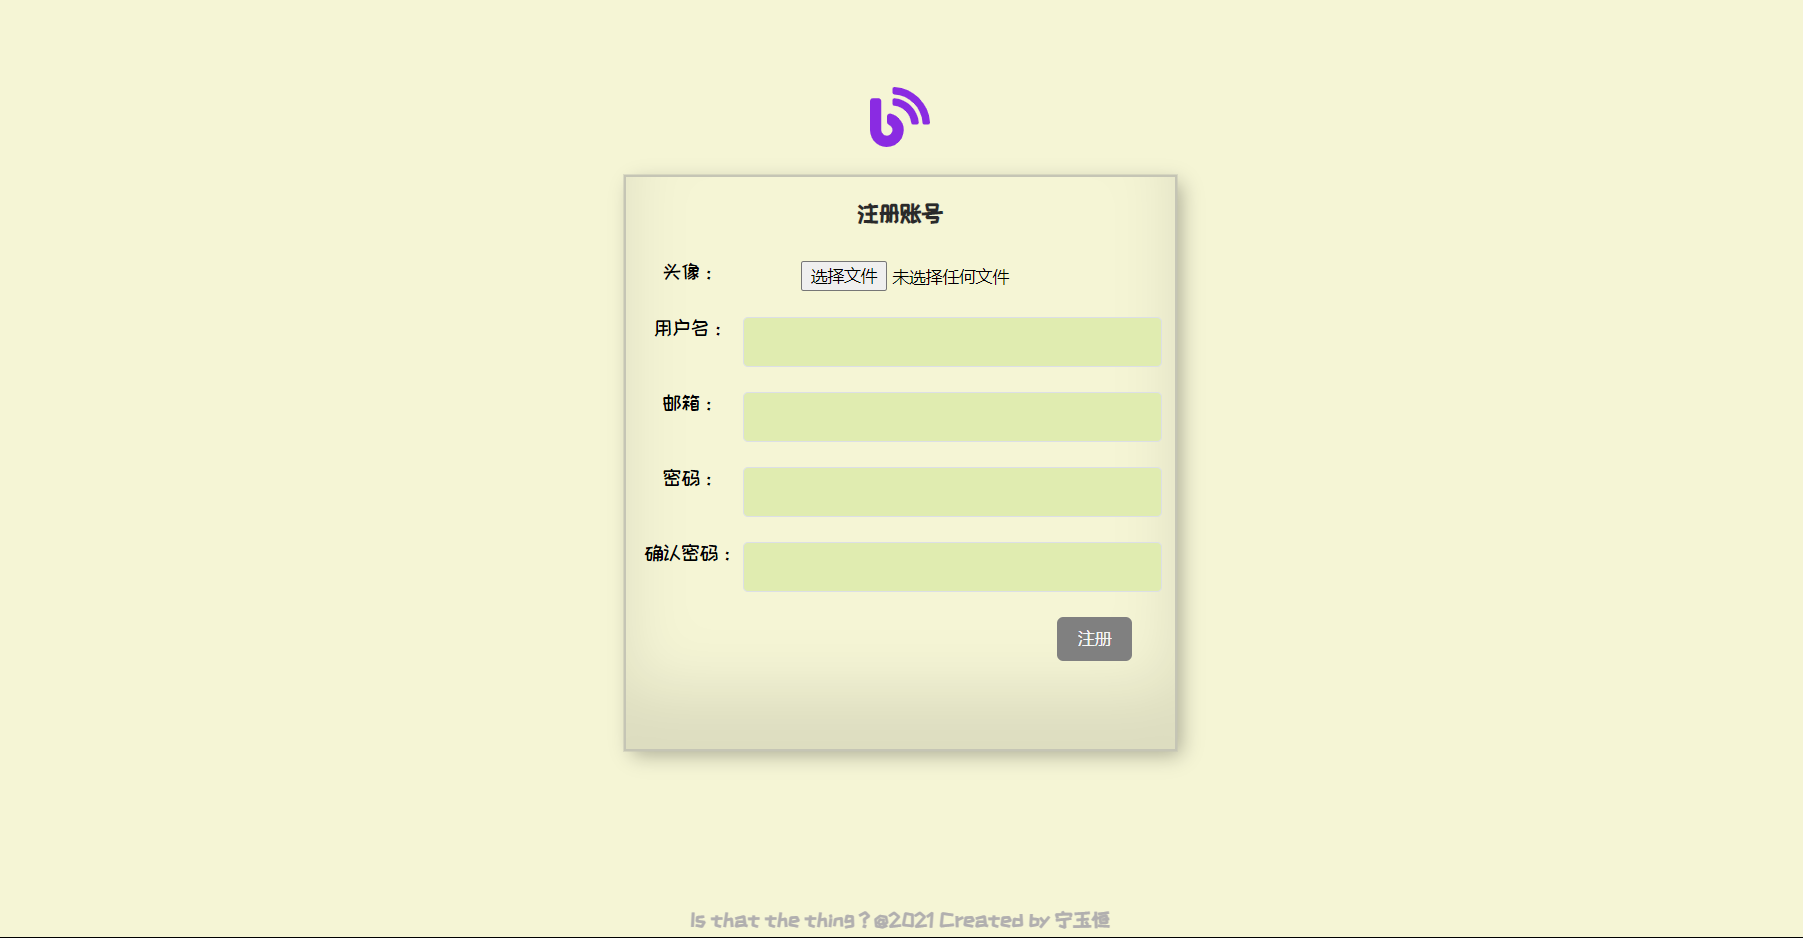
\includegraphics[scale=0.35]{figure/register}
	\caption{注册页}
\end{figure}

\subsection{登录}
在首页点击右上角登录按钮,即可访问登录页,输入注册的邮箱及密码.

\begin{figure}[thbp!]
	\centering
	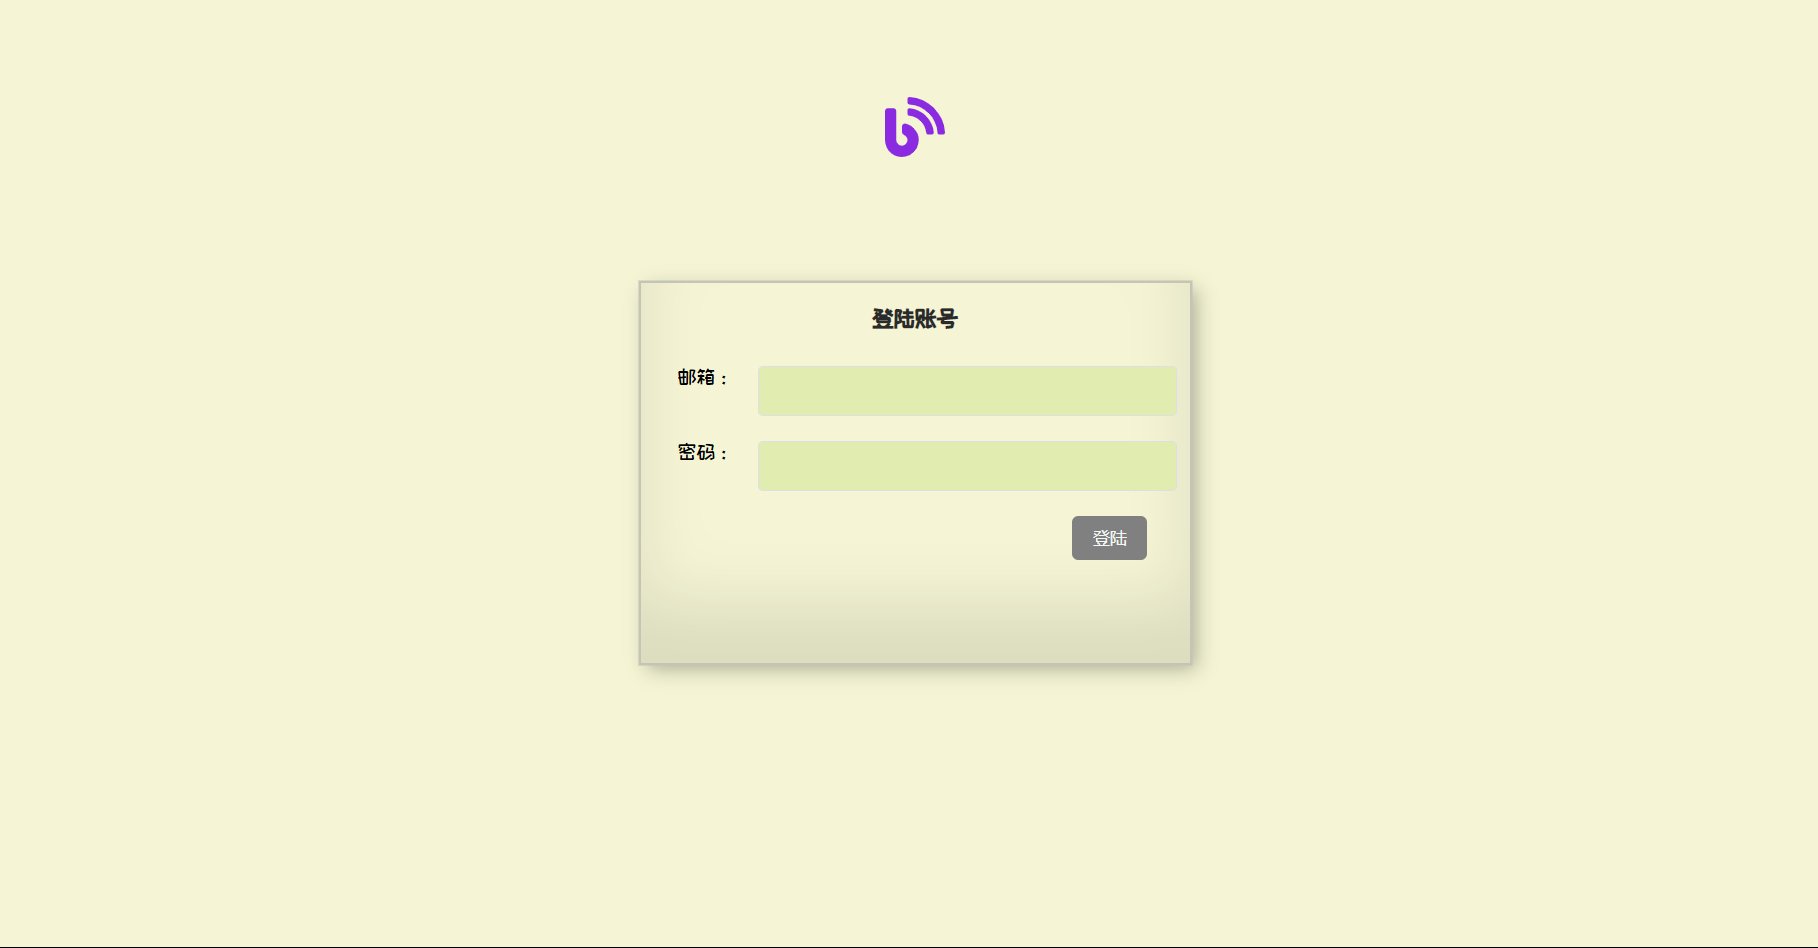
\includegraphics[scale=0.35]{figure/login}
	\caption{登录页}
\end{figure}

      %
\section{文章访问}

\subsection{访问登录状态下主界面}
在完成登录以后点击页面上方导航栏后回到主页,可以看到文章名称,发布日期,标签,作者等信息.

\begin{figure}[thbp!]
	\centering
	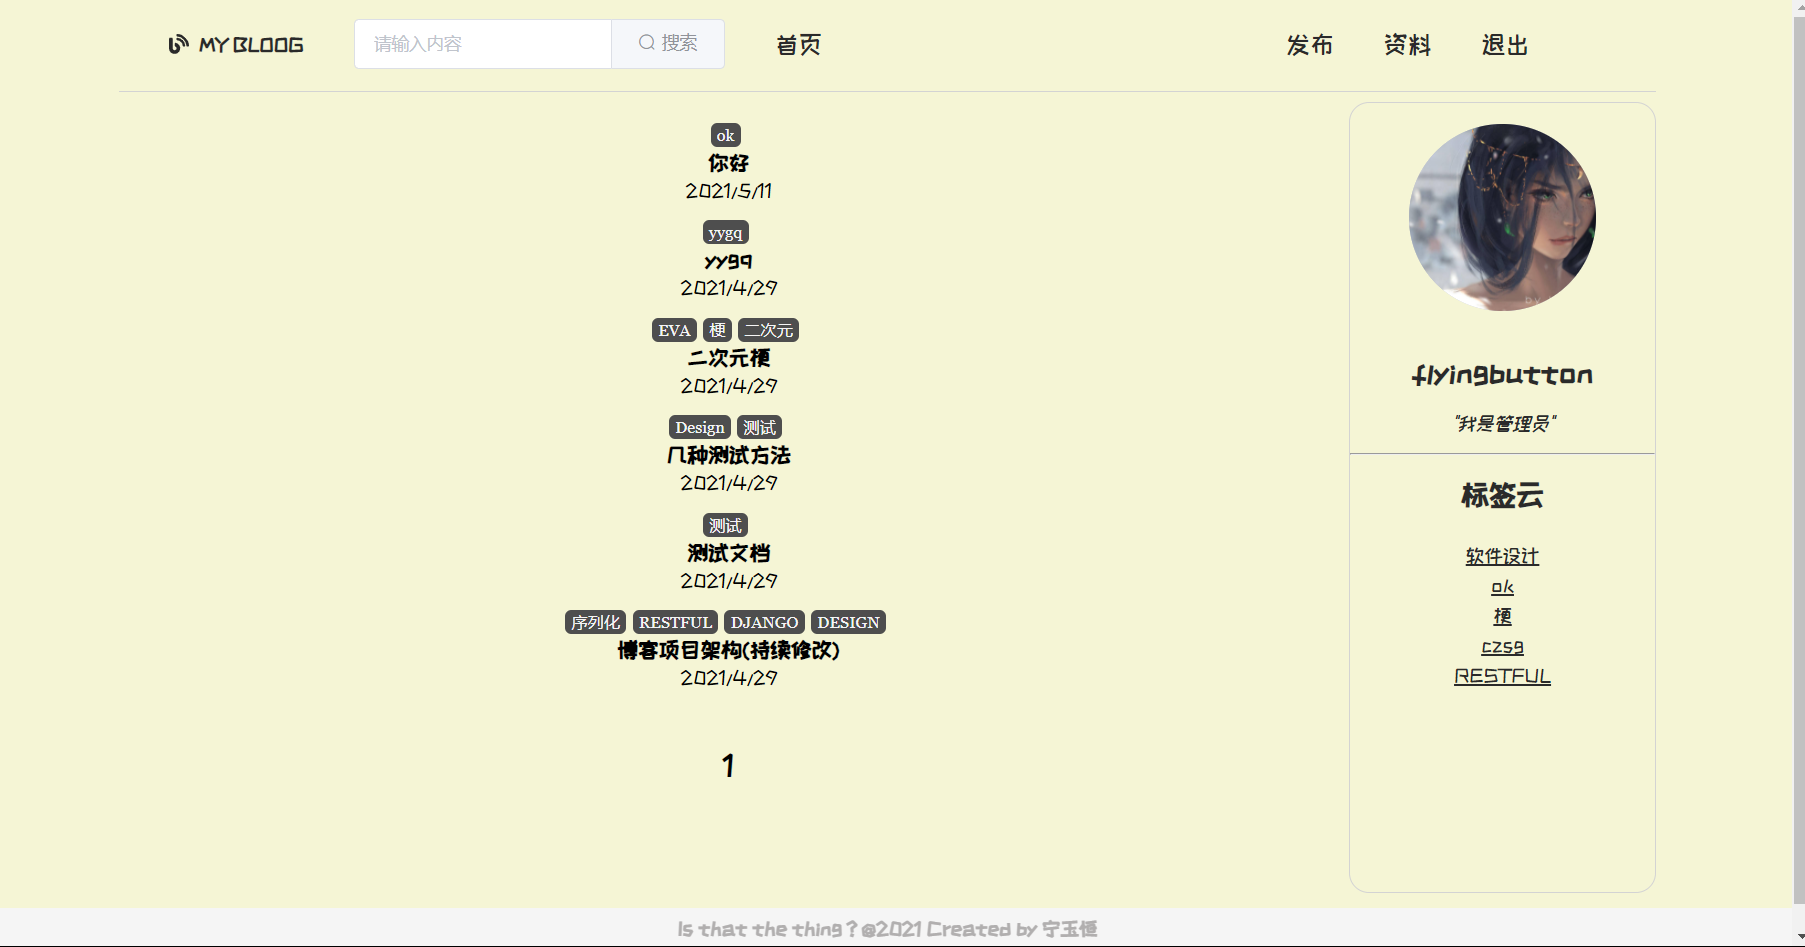
\includegraphics[scale=0.35]{figure/home_page_login}
	\caption{登录后的主界面}
\end{figure}

\subsection{访问非登录状态下主界面}
在点击退出登陆后,则以游客身份访问主界面.

\begin{figure}[thbp!]
	\centering
	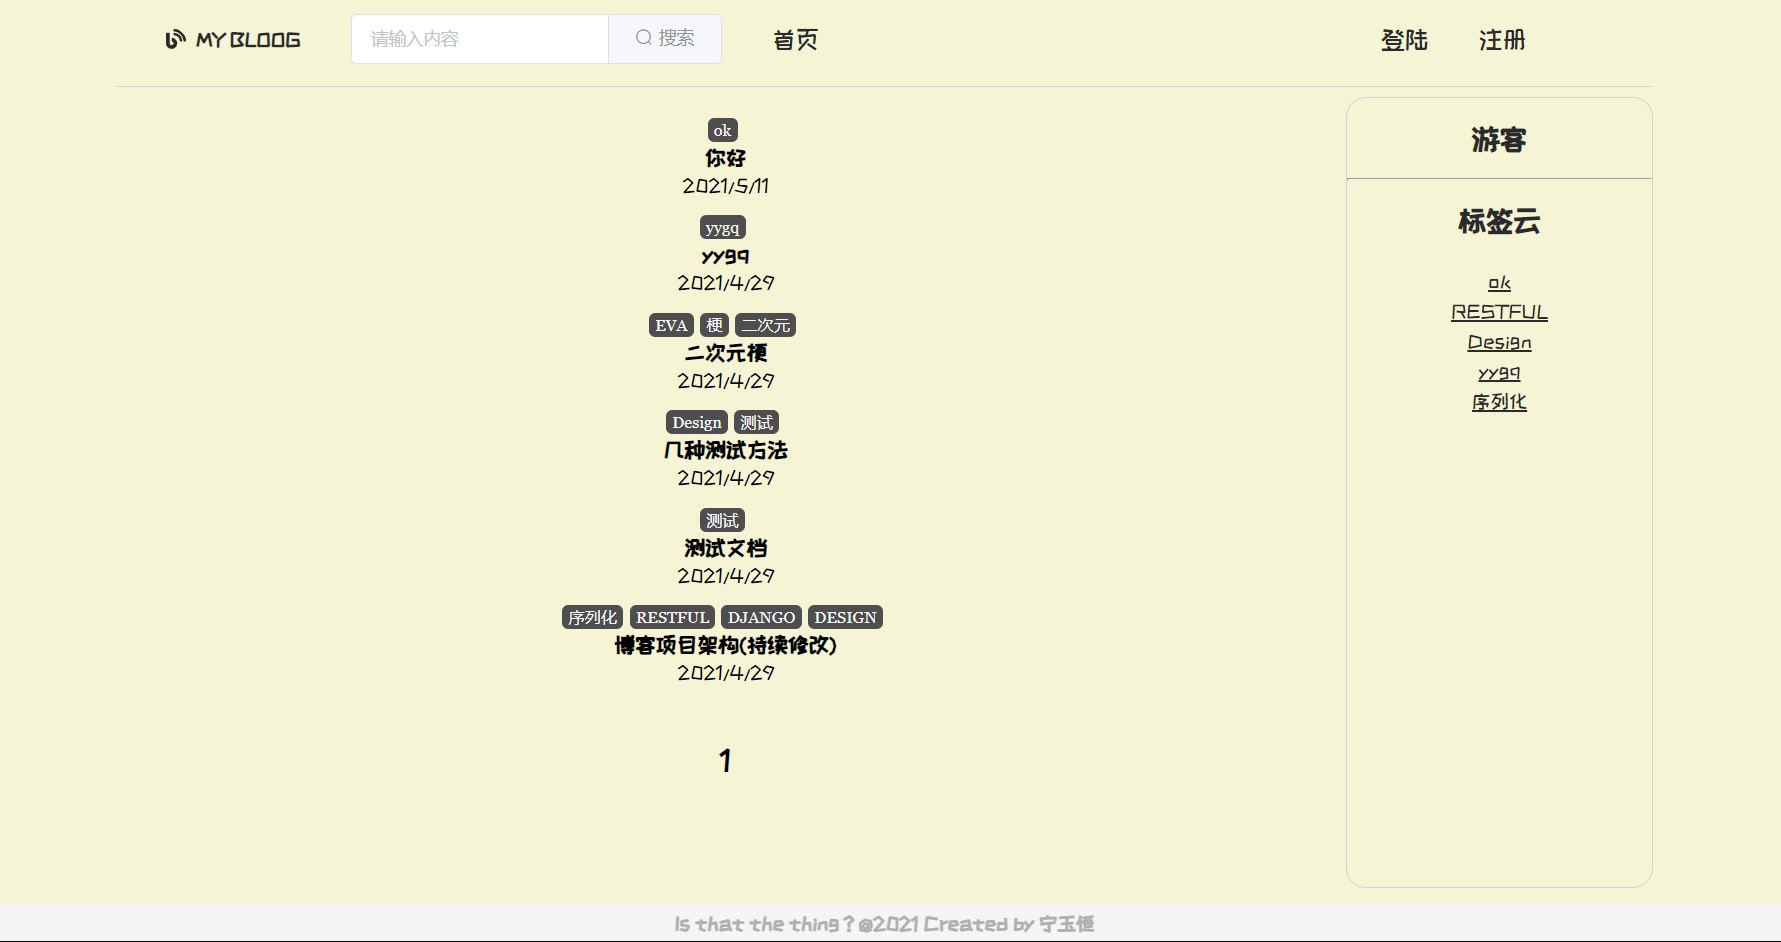
\includegraphics[scale=0.35]{figure/home_page_guest}
	\caption{未登录时的主界面}
\end{figure}


\section{文章增删改}

\subsection{文章详情}

点击主界面的文章链接,即可访问文章详情页.
\begin{figure}[thbp!]
	\centering
	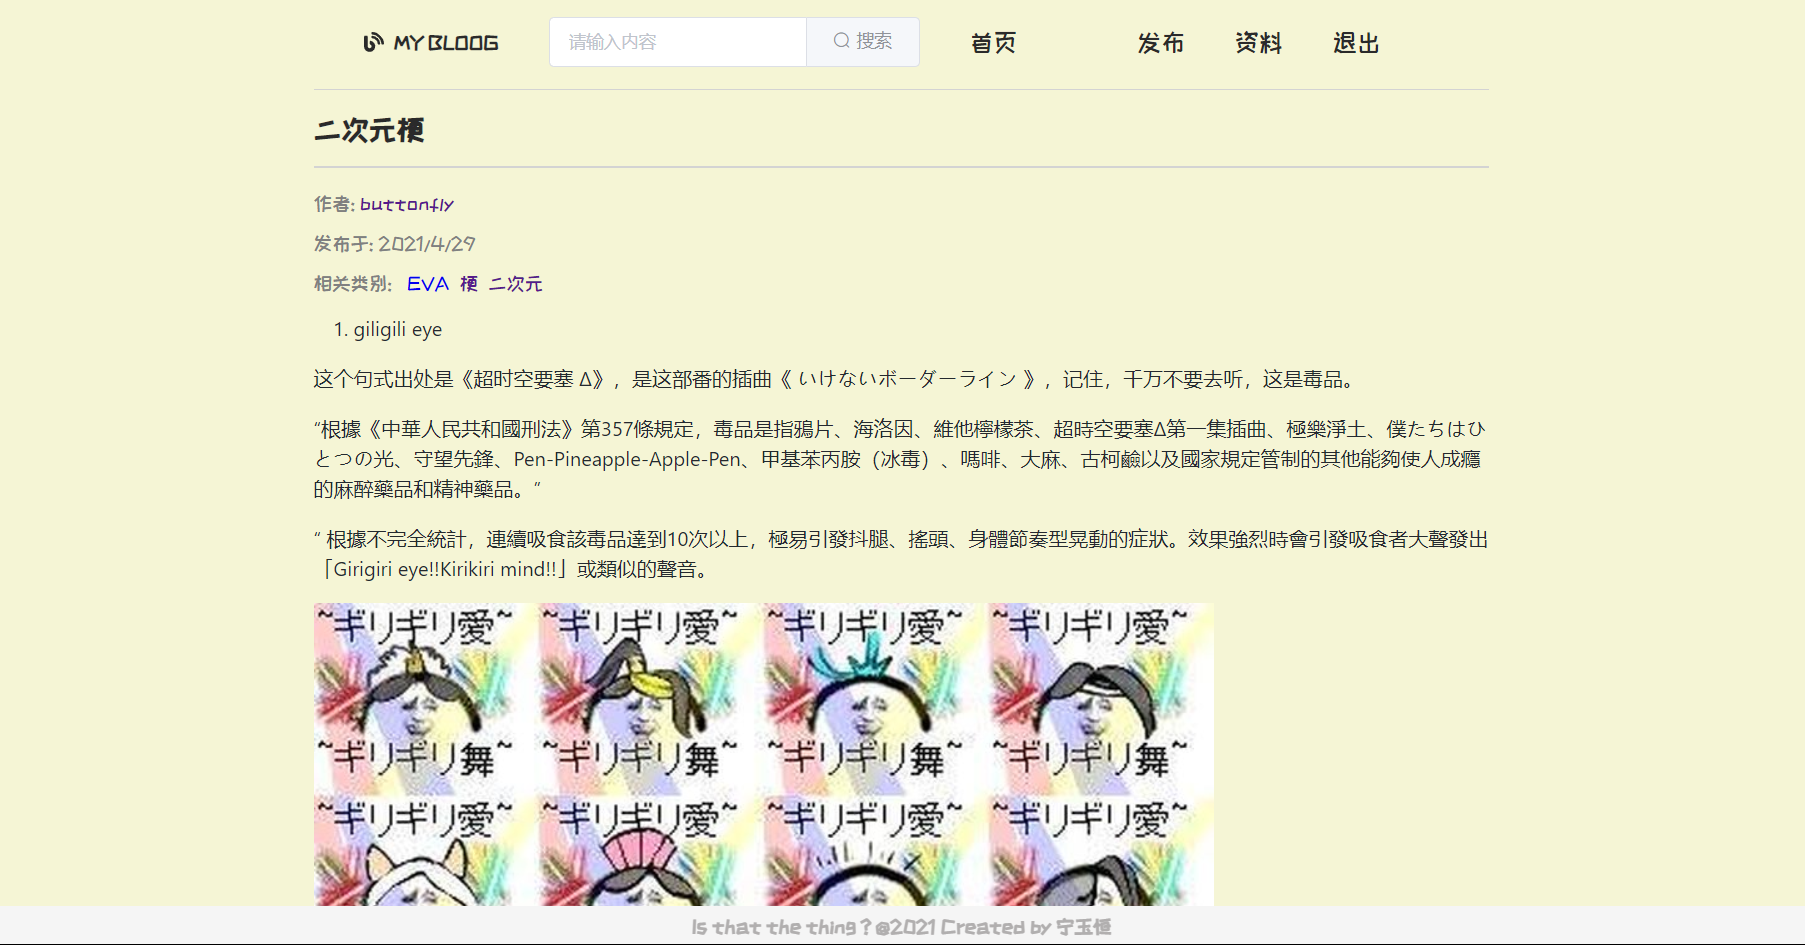
\includegraphics[scale=0.35]{figure/article1}
	\caption{详情页完美支持markdown语法显示}
\end{figure}

\begin{figure}[thbp!]
	\centering
	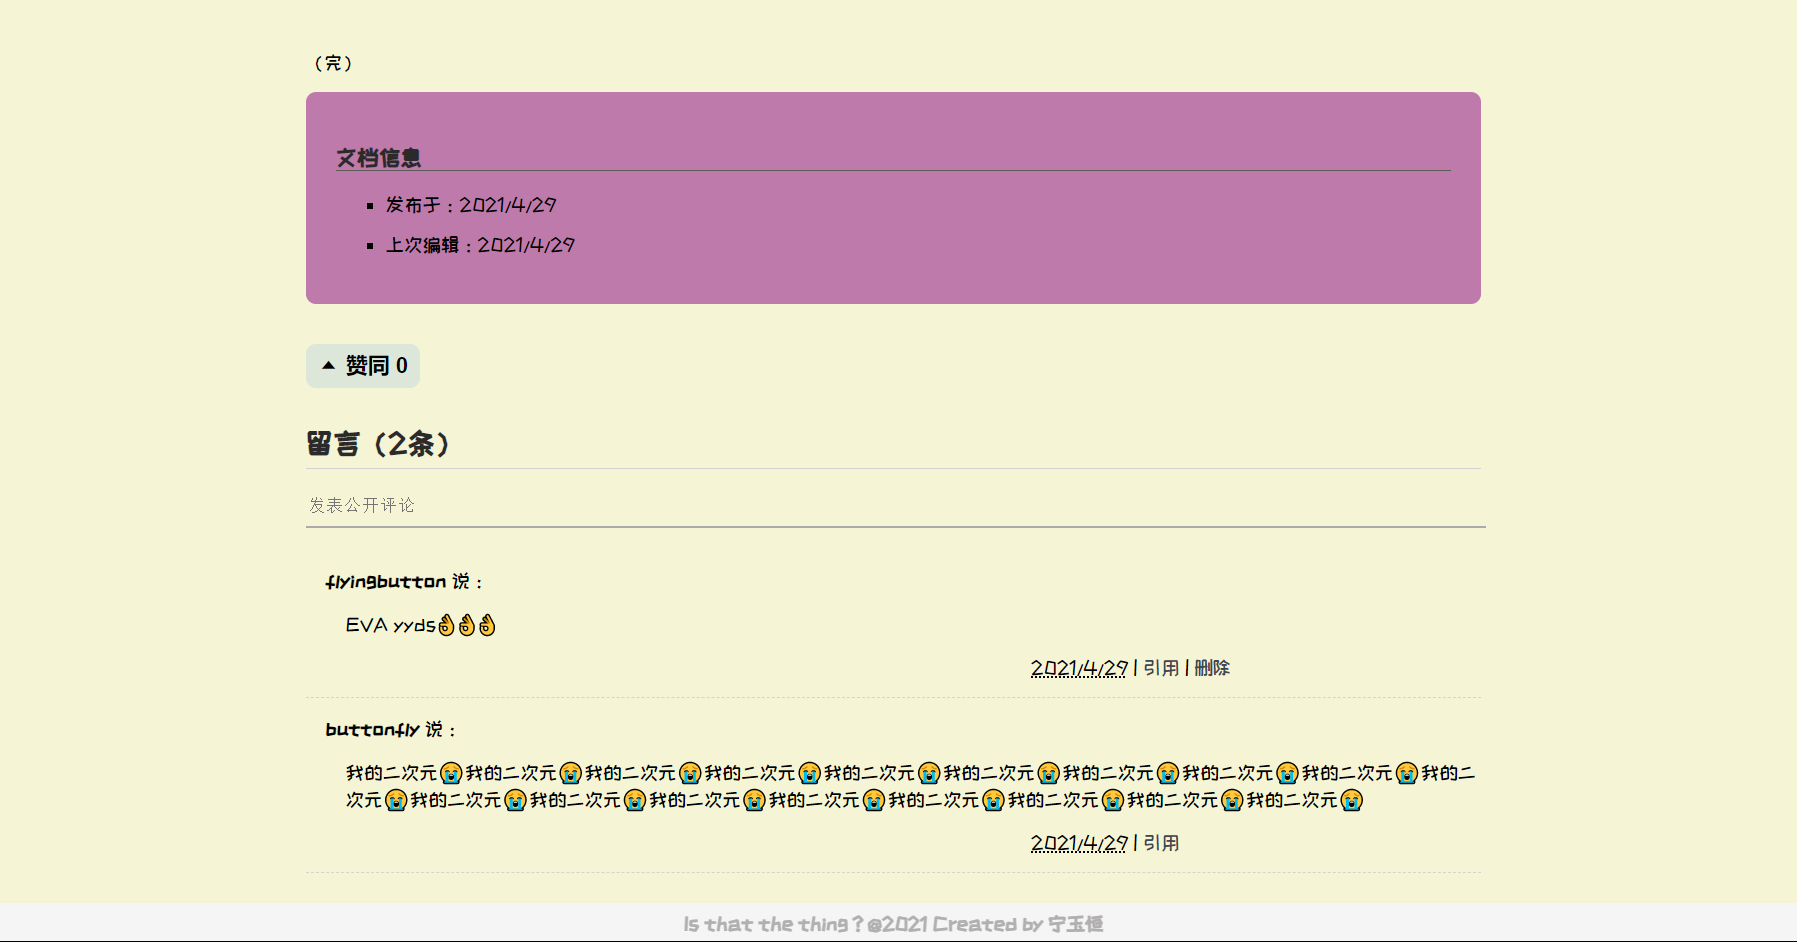
\includegraphics[scale=0.35]{figure/article2}
	\caption{文章支持点赞,留言支持嵌套}
\end{figure}

\subsection{文章发布或删改}

点击界面上方导航栏的发布按钮,即可进入到新文章的编辑.
\begin{figure}[thbp!]
	\centering
	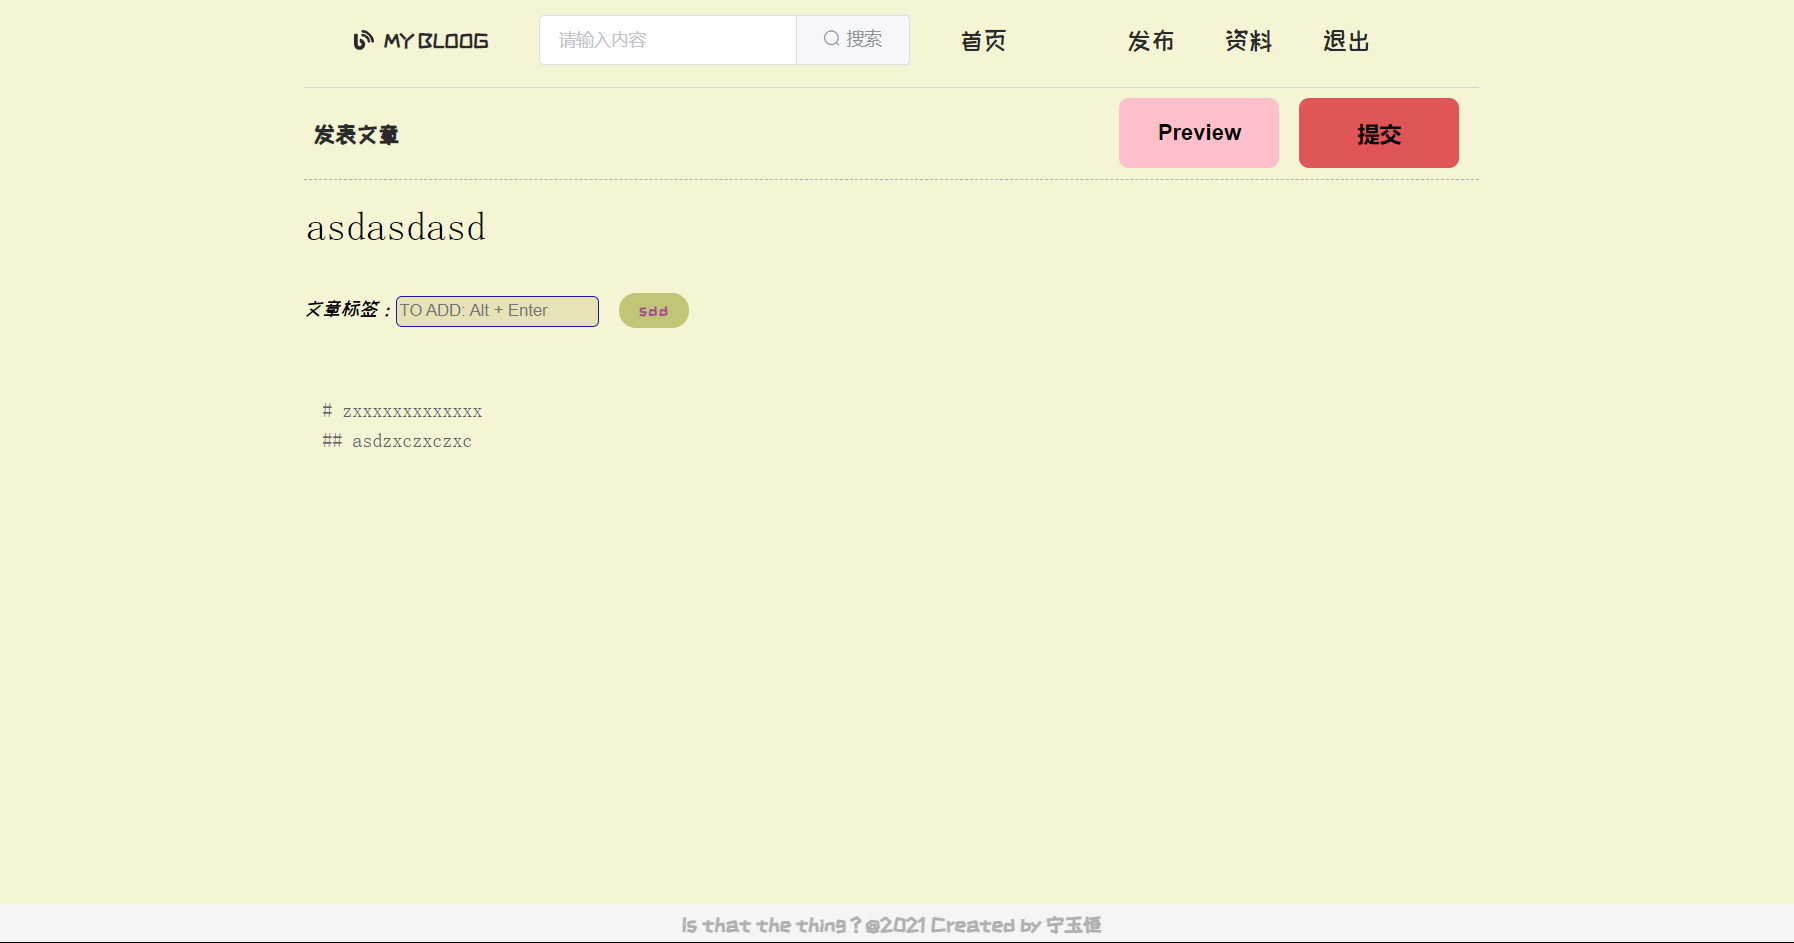
\includegraphics[scale=0.35]{figure/new}
	\caption{文章编辑支持markdown语法,且支持预览,可自定义添加标签}
\end{figure}

修改页面与之类似.
\begin{figure}[thbp!]
	\centering
	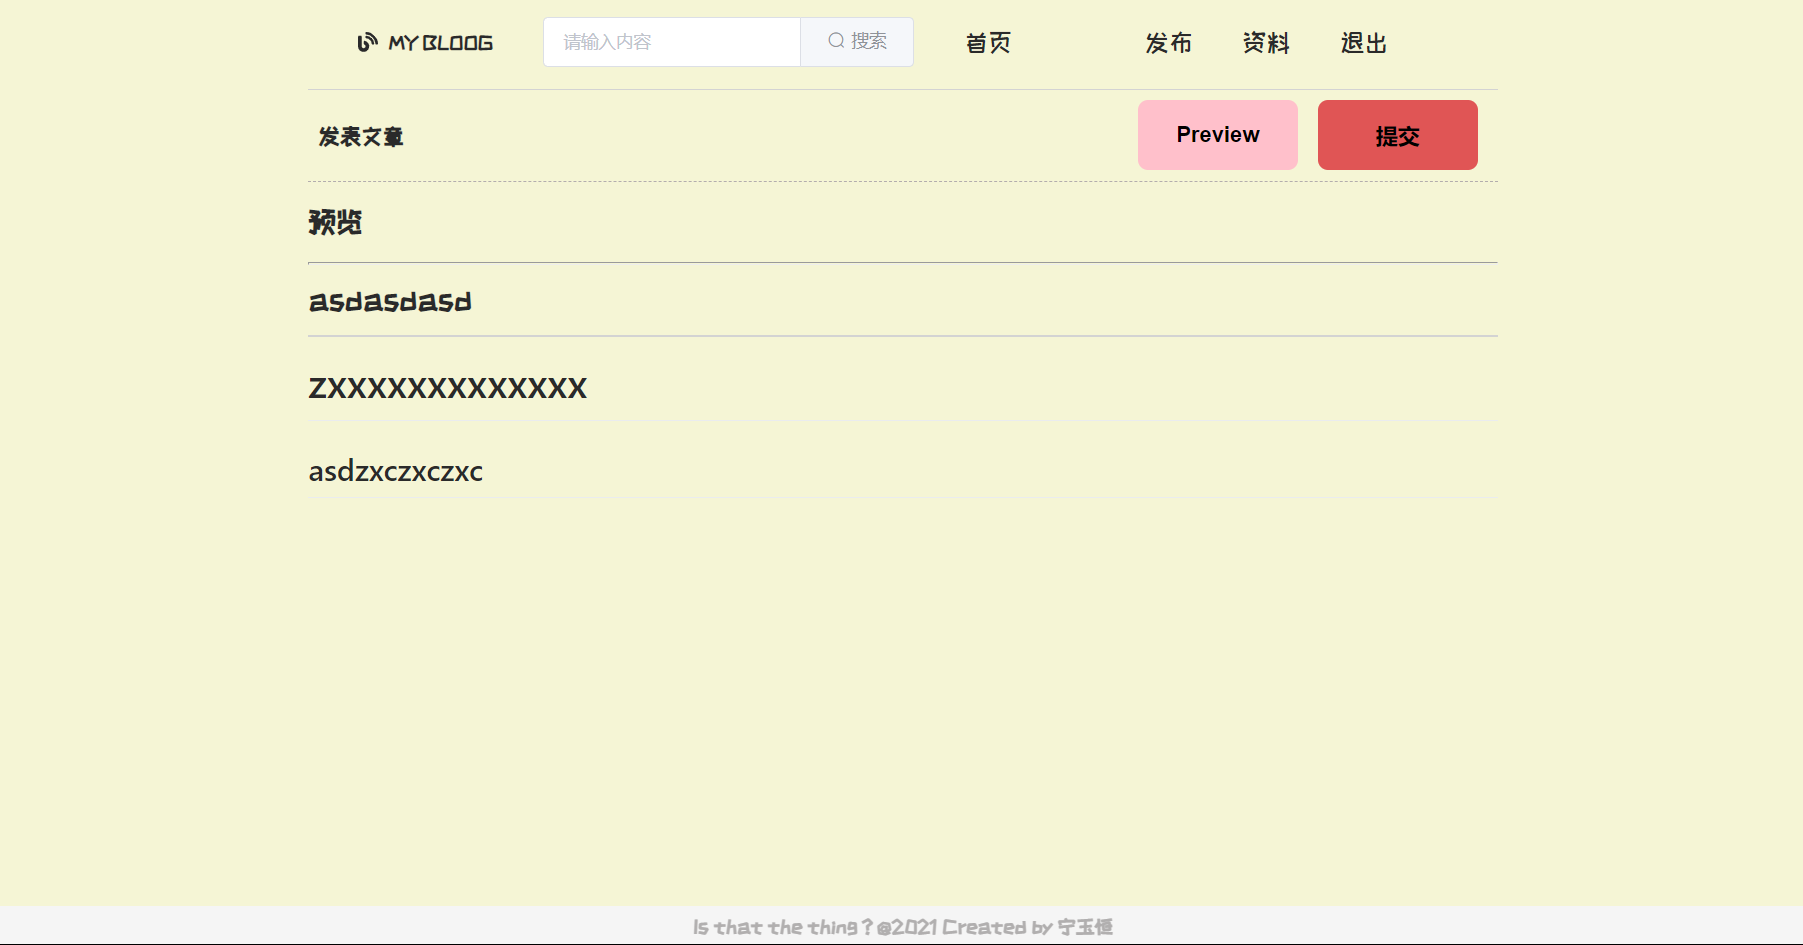
\includegraphics[scale=0.35]{figure/modify}
	\caption{文章内容修改}
\end{figure}


\section{模型求解}
\section{已5未来发展}
\subsection{已知问题}
本模板未采用2013版规范的页边距设置,因为实在是办不到2.5CM顶部页边距加上2.6CM的页眉设置啊。
\subsection{未来发展}
武汉理工大学本科生论文的未来发展还是需要各位用户的参与,如果每一个用户都能贡献出一点关于\LaTeX 模板的想法和意见,我相信几年之后武汉理工大学本科生论文模板会成为其他高校学习和借鉴的例子。同学当自强,让我们一起来丰富完善这个模板,如果你有很好的建议或者意见请发送到 thesis@tsaoyu.com
\subsection{官方认证}
到目前为止(\today )没有武汉理工大学任何官方组织对于本模板的格式或者内容进行认证,这代表采用本模板进行的论文写作可能不被官方的论文系统接受。如在进行原创性(防抄袭)检测的时候,可能需要提供提供doc版本的论文。希望用户了解到这个潜在的风险,做好文件转换和备份的准备。本人不对任何由于使用本模板而导致的毕业论文纠纷承担任何责任!
\section{附件}

\subsection{本地文件}

\begin{itemize}
	\item training.py:     训练模型代码
	\item training.ipynb:  代码同training.py,保存了输出内容
	\item inference.py:    使用模型进行预测代码
	\item inference.ipynb: 代码同inference.py,保存了输出内容
	\item result.csv:      保存了预测结果,raw\_id对应音频文件名,birds用空格分隔检测出的鸟类,鸟类名为\href{ebird.org}{ebird.org}中编码的,需要查看其学名可以通过访问ebird.org/species/[鸟名编码],在banner图片中查看到.如图所示:
	\begin{figure}[thbp!]
		\centering
		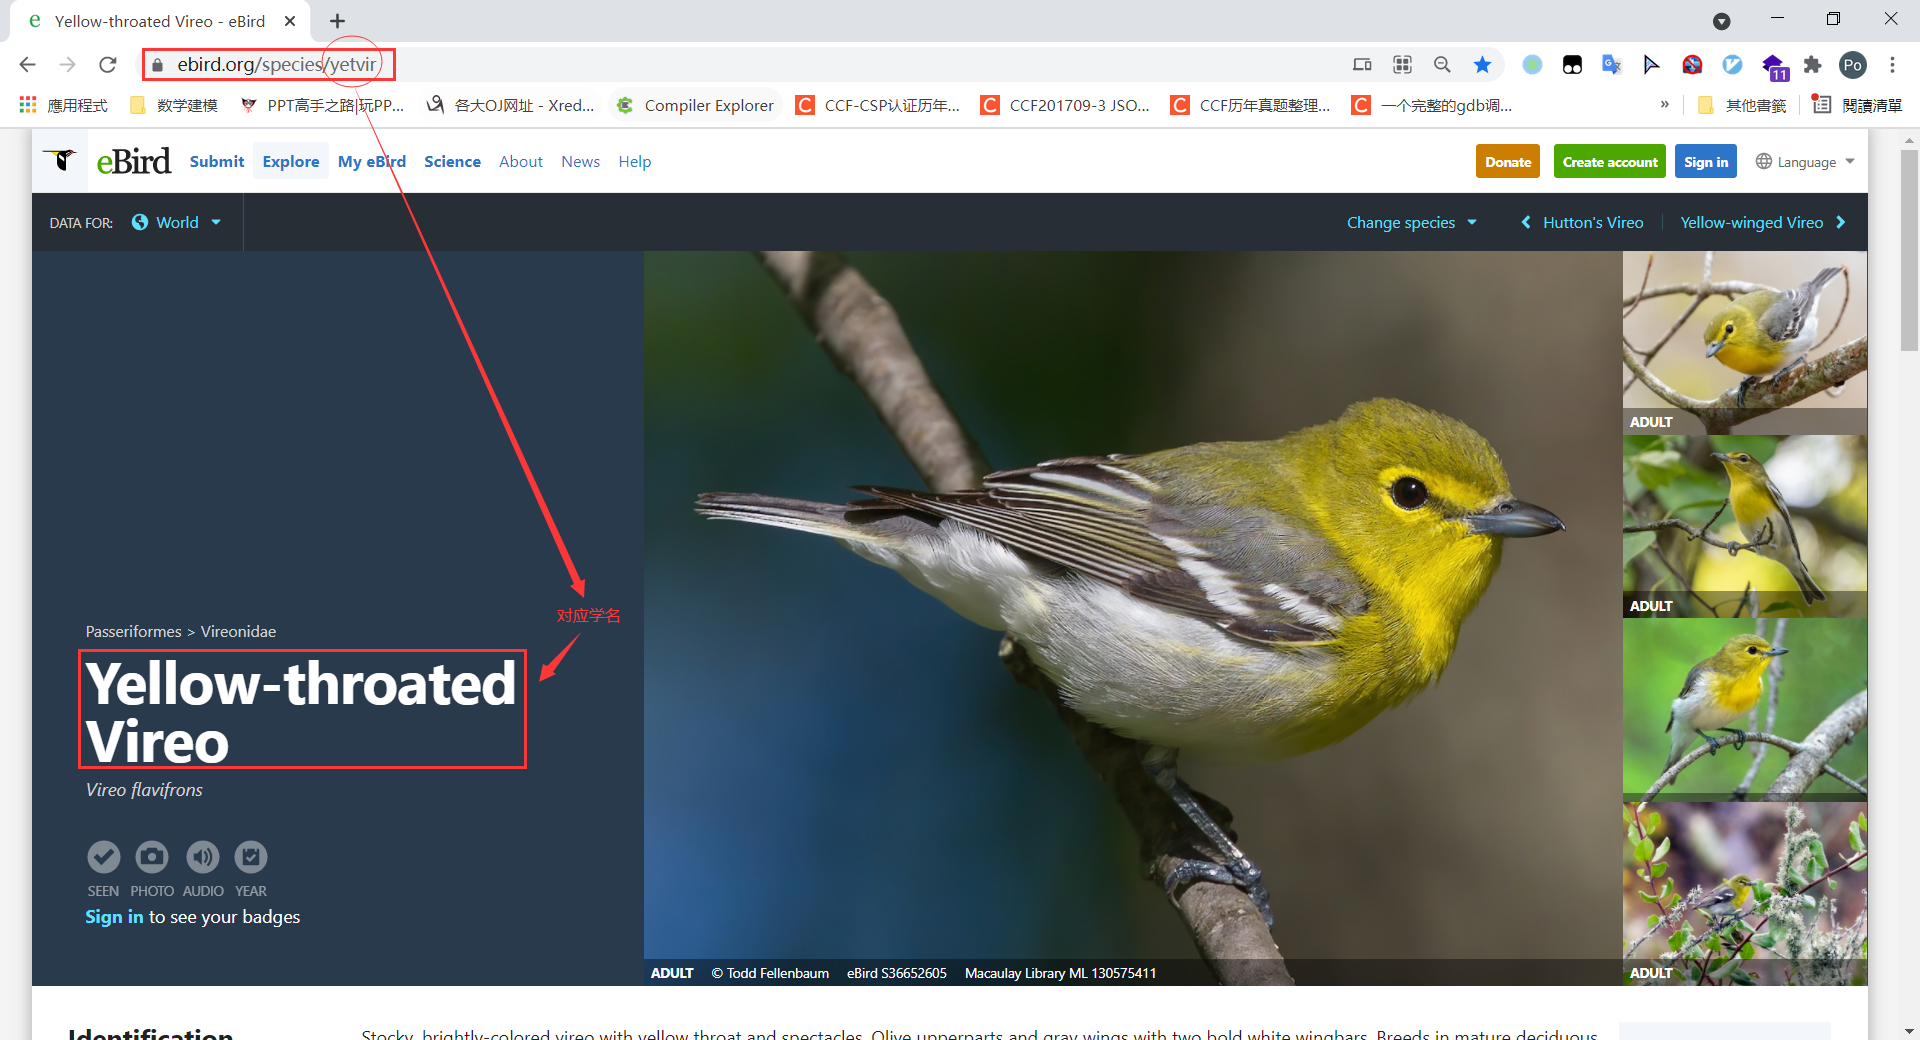
\includegraphics[scale=0.2]{figure/find_name}
		\caption{查看yetvir对应的学名为Yellow-throated Vireo}
	\end{figure}
\end{itemize}

\subsection{在线数据(点击文字超链接可达)}

\begin{itemize}
	\item \href{https://www.kaggle.com/c/birdsong-recognition}{Cornell Birdcall Identification鸟类识别比赛数据库}
	\item \href{https://www.kaggle.com/tsuipo/bird-pic}{自行从\href{ebird.org}{ebird.org}爬取后上传的鸟类图片}
\end{itemize}
%============= 参考文献 =====================
\addcontentsline{toc}{section}{参考文献}
\bibliography{bibfile}
\clearpage
%=============  致谢  ======================
\section*{致谢}
\addcontentsline{toc}{section}{致谢}
感谢父母为我提供的良好的衣食条件,让我有精力投入到这项没有经济回报的项目中去。
感谢徐海祥老师为我定制的论文题目,这个题目让我有兴趣制作这个模板。感谢武汉理工大学博士与硕士论文作者Hu,Weiyi,我在本模板制作的过程中参考了前辈的思路的方法。我研究过的模板还包括:上海交通大学,清华大学,哈尔滨工业大学,以及中国科技大学。其中论文引用格式GBT7714-2005-BibTeX-Style是上海财经大学的Haixing Hu作品,本模板离不开这些有益的资源的支持。同样感谢正在使用这个模板的你,相信通过你们的使用和传播,这个模板会变得越来越完善。
%\newpage
%\appendix
%
%%%附录第一个章节
%\section{第一附录}
%
%
%%%变量列举
%
%\begin{table}[H]
%\caption{Symbol Table-Constants}
%\centering
%\begin{tabular}{lll}
%\toprule
%Symbol & Definition  & Units\\
%\midrule[2pt]
%\multicolumn{3}{c}{\textbf{Constants} }\\
%$DL$&Expectancy of poisson-distribution &  unitless \\
%$NCL$ &Never- Change-Lane& unitless\\
%$CCL$&Cooperative-Change-Lane& unitless\\
%$ACL$&Aggressive-Change-Lane& unitless\\
%$FCL$&Friendly-Change-Lane& unitless\\
%$SCC$&Self-driving-Cooperative-Car& unitless\\
%$NSC$&None-Self-drive-Car& unitless\\
%\bottomrule
%\end{tabular}
%\end{table}
%
%
%\section{第二附录}
%\textcolor[rgb]{0.98,0.00,0.00}{\textbf{Simulation Code}}
%\begin{python}
%import java.util.*;  
%public class test {  
%    public static void main (String[]args){   
%        int day=0;  
%        int month=0;  
%        int year=0;  
%        int sum=0;  
%        int leap;     
%        System.out.print("请输入年,月,日\n");     
%        Scanner input = new Scanner(System.in);  
%        year=input.nextInt();  
%        month=input.nextInt();  
%        day=input.nextInt();  
%        switch(month) /*先计算某月以前月份的总天数*/    
%        {     
%        case 1:  
%            sum=0;break;     
%        case 2:  
%            sum=31;break;     
%        case 3:  
%            sum=59;break;     
%        case 4:  
%            sum=90;break;     
%        case 5:  
%            sum=120;break;     
%        case 6:  
%            sum=151;break;     
%        case 7:  
%            sum=181;break;     
%        case 8:  
%            sum=212;break;     
%        case 9:  
%            sum=243;break;     
%        case 10:  
%            sum=273;break;     
%        case 11:  
%            sum=304;break;     
%        case 12:  
%            sum=334;break;     
%        default:  
%            System.out.println("data error");break;  
%        }     
%        sum=sum+day; /*再加上某天的天数*/    
%        if(year%400==0||(year%4==0&&year%100!=0))/*判断是不是闰年*/    
%            leap=1;     
%        else    
%            leap=0;     
%        if(leap==1 && month>2)/*如果是闰年且月份大于2,总天数应该加一天*/    
%            sum++;     
%        System.out.println("It is the the day:"+sum);  
%        }  
%} 
%\end{python}
%
%


\end{document}
%%%%%%%%%% 结束 %%%%%%%%%%